\documentclass[UTF8]{ctexart}
\usepackage{bookmark}
\usepackage{geometry}
\usepackage{hyperref}
\geometry{a4paper,scale=0.8}
\usepackage{ctex}
\usepackage[style=caspervector,backend=biber,utf8]{biblatex}
\usepackage{booktabs}
\usepackage{array}
\usepackage{fancyhdr}
\pagestyle{fancy}
\fancyhf{}
\renewcommand\footrulewidth{1pt}
\lhead{王铠泽}
\rhead{PB18020766}
\chead{\href{mailto:volar@mail.ustc.edu.cn}{volar@mail.ustc.edu.cn}}
\rfoot{中国科学技术大学}
\lfoot{\today}
\usepackage{graphicx}
\usepackage{float}
\usepackage{subfigure}


\begin{document}

	\centering\textbf{\LARGE{计算物理A第五次作业}}
	
	
	王铠泽\qquad PB18020766
	
		
	\section{作业题目}
	
	\begin{itemize}
		\item 对于球面上均匀分布的随机坐标点,给出它们在$(x,y)$平面上投影的几
		率分布函数。并由此验证$Marsaglia$抽样方法确为球面上均匀分布的随机抽样。
		\item $Marsaglia$抽样
		$$\left\{
		\begin{array}{lc}
			x=2u\sqrt{1-r^2}\\
			y=2v\sqrt{1-r^2}\\
			z=1-2r^2\\
		\end{array}
		\right.$$
	其中,$u,v$为$[-1,1]$上均匀分布随机数。
	\end{itemize}
	
	\section{实现方法}
	
	\begin{itemize}
		\item 变换抽样法
		
		球坐标和直角坐标转化:
		$$ \left\{
		\begin{array}{l}
		x=sin\theta cos\phi\\
		y=sin\theta sin\phi\\
		z=cos\theta\\
		\end{array} \right. $$
		
		当球面上均匀分布$f(\theta,\phi)=\frac{1}{4\pi}sin\theta$要变换到二维$x-y$上时:
		$$f(\theta,\phi)d\theta d\phi=g(x,y)dxdy$$
		从而有(考虑到两个上下半球在$x-y$平面投影一致):
		$$g(x,y)=\frac{1}{2\pi}\vert \frac{\partial(\theta,\phi)}{\partial(x,y)}\vert=\frac{1}{2\pi}\frac{1}{\sqrt{1-s^2}}$$
		其中$s=\sqrt{x^2+y^2}$
		
		而对于$Marsaglia$抽样的变换,有:
		$$\vert \frac{\partial(x,y)}{\partial(u,v)}\vert=4|1-2(u^2+v^2)|=4|1-2r^2|=4\sqrt{1-s^2}$$
		但这里有个小细节,当$r^2=u^2+v^2=\frac{1}{2}$时$Jacobi$行列式为0,有间断。而$r^2=\frac{1}{2}$刚好可以将圆盘分为等面积的两个部分,将这两部分分开讨论,将会导致最后的概率密度乘上因子2。另一方面,由于舍选导致$p(u,v)=\frac{1}{\pi}$,而不是$\frac{1}{4}$。
		$$\Rightarrow g'(x,y)=2p(u,v)\cdot\frac{\partial(u,v)}{\partial(x,y)}=\frac{1}{2\pi}\frac{1}{\sqrt{1-s^2}}=g(x,y)$$
		
		这就验证了$x-y$平面上的分布。
		
		接下来验证$x-z$平面分布($y-z$分布和这个类似,不再证明)
		$$f(\theta,\phi)=h(x,z)dxdz$$
		$$\Rightarrow h(x,z)=\frac{1}{2\pi}\vert \frac{\partial(\theta,\phi)}{\partial(x,z)}\vert=\frac{1}{2\pi}\frac{1}{\sqrt{1-z^2-x^2}}$$
		
		而$Marsaalia$对应的密度函数$h'$满足:
		$$h'(x,y)=2p(u,v)\cdot\frac{\partial(u,v)}{\partial(x,z)}=\frac{1}{4\pi}\frac{1}{v\sqrt{1-u^2-v^2}}$$
		
		另一方面:
		$$\frac{1}{\sqrt{1-z^2-x^2}}=\frac{1}{2}\frac{1}{v\sqrt{1-u^2-v^2}}$$
		
		$$\Rightarrow h'(x,y)=h(x,y)$$
		
		至此,证毕。事实上$x,y,z$三个方面应当是等价的,所以$x-y,y-z,z-x$平面上的分布应当是一样的。
		下面给出随机数在二维平面上的结果
	\end{itemize}
	
	\section{程式说明}
	\begin{itemize}
		\item Marsaglia.c
		
		该程式使用$Marsaglia$抽样方法抽取三维球面上均匀分布随机数。
		
		\item rdm.h
			
		这是一个包含了使用16807产生器生成指定长度的$[0,1]$上均匀分布随机数函数的头文件。
		
		\subitem void rdm(int N,double *x,int method)
		
		该函数将输入的指针$x$对应的长度为$N$的数组用$[0,1]$上的随机数填满。method是关于初始种子的选择。method=0:默认种子;method=1,时间种子。
		
		\item dimensions.c 
		
		该程式是后续探究其他维度球面均匀分布时给出随机数的函数(二维,四维)。
		
		\item time\_seed0.txt
		
		$Marsagli.c$抽样时对应的时间种子数据(1个种子)。
		
		\item time\_seed.txt
		
		$dimensions.c$抽样时对应的时间种子数据(4个种子)。
		
		\item sphere\_surface.txt,ring.txt,4-sphere.txt
		
		这些都是数据文件。
	\end{itemize}
	
	\section{计算结果}

%	\begin{figure}[H]
%	\centering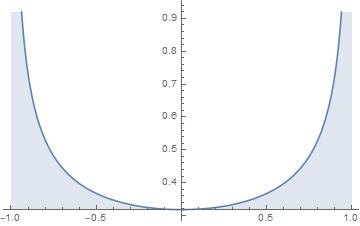
\includegraphics[width=2in]{1.jpg}
%	\caption{something}\label{fig:1}
%	\end{figure}
	
	\begin{figure}[H]
		\centering  %图片全局居中
		\subfigure[直接抽样$x-y$平面分布]{
			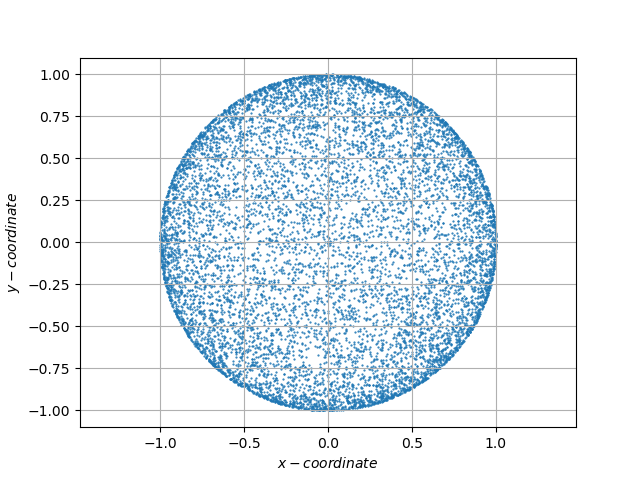
\includegraphics[width=0.48\textwidth]{../x-y.png}}
		\subfigure[$Marsaglia$抽样$x-y$平面分布]{
			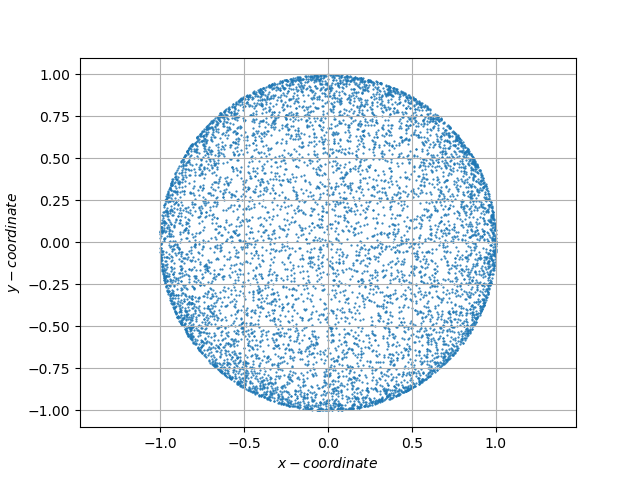
\includegraphics[width=0.48\textwidth]{../M-x-y.png}}
		\subfigure[直接抽样$x-z$平面分布]{
			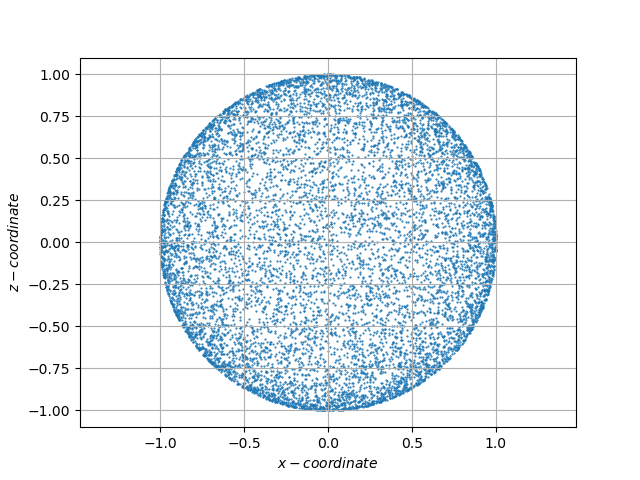
\includegraphics[width=0.48\textwidth]{../x-z.png}}
		\subfigure[$Marsaglia$抽样$x-z$平面分布]{
			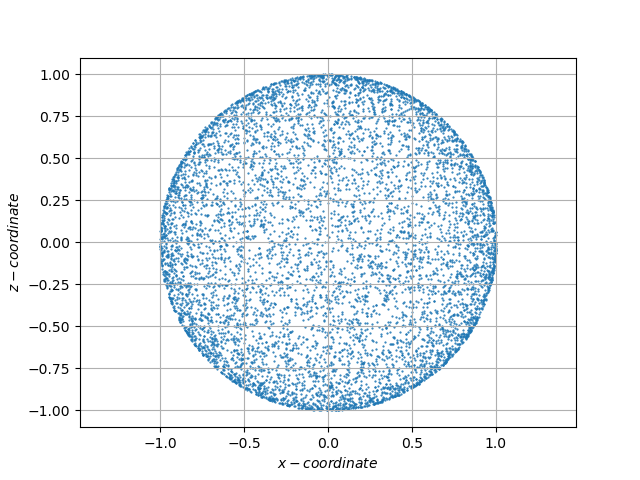
\includegraphics[width=0.48\textwidth]{../M-x-z.png}}
		\caption{抽样分布}
		\label{N}
	\end{figure}
	
	
	\begin{flushleft}
		可以看出,球面上的均匀分布投影到二维平面上体现出外围密集(边缘发散),中间稀疏的特征。这是和二维平面上有:
	$g(x,y)=\frac{1}{2\pi}\frac{1}{\sqrt{1-s^2}}$
	是吻合的

	另一方面,这也直观上验证了$Marsaglia$抽样和直接抽样效果是一样的,只是牺牲了效率。
	
%		\begin{figure}[H]
%			\centering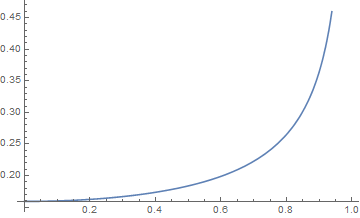
\includegraphics[width=3.5in]{../func.png}
%			\caption{$h(r)$函数图像}
%		\end{figure}
	\end{flushleft}
	\clearpage
	\section{其他}
	
\begin{flushleft}
		可以考虑其他维度的$Marsaglia$抽样:
\end{flushleft}
\begin{flushleft}
	\textbf{	二维:}
\end{flushleft}
		\begin{figure}[H]
			\centering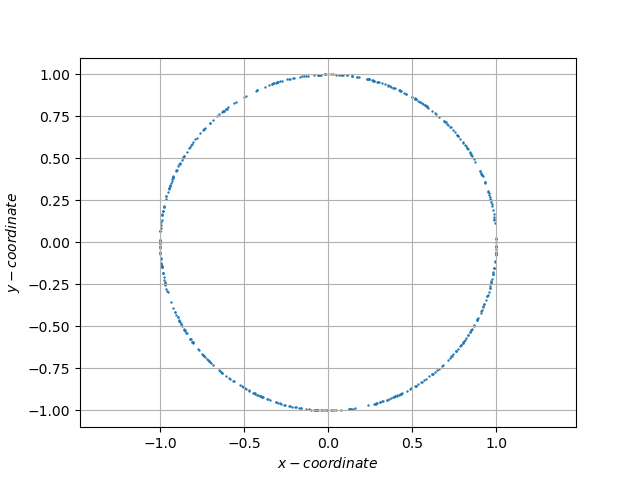
\includegraphics[width=4in]{../2-xy}
			\caption{二维球面均匀分布}
		\end{figure}
\begin{flushleft}
		和意料之中差别不大。
\end{flushleft}
	\clearpage
\begin{flushleft}
		\textbf{四维:}
\end{flushleft}
		\begin{figure}[H]
			\centering  %图片全局居中
			\subfigure[$N=10000$三维投影]{
				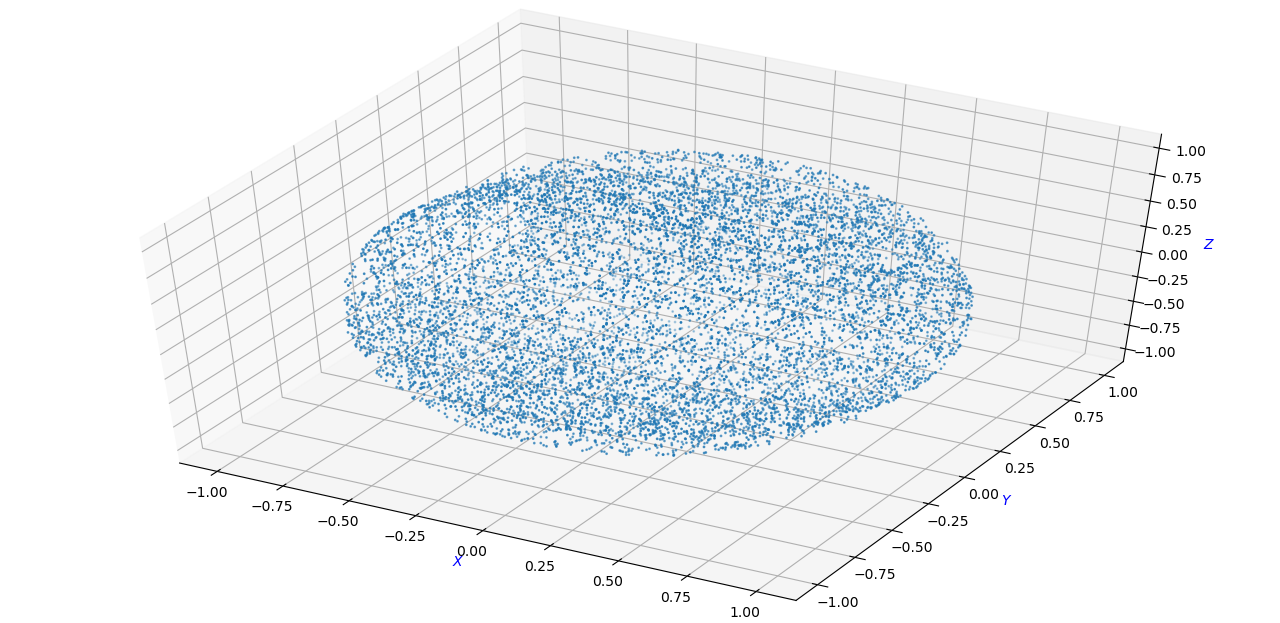
\includegraphics[width=0.45\textwidth]{../4-xyz-1w.png}}
			\subfigure[$N=50000$三维投影]{
				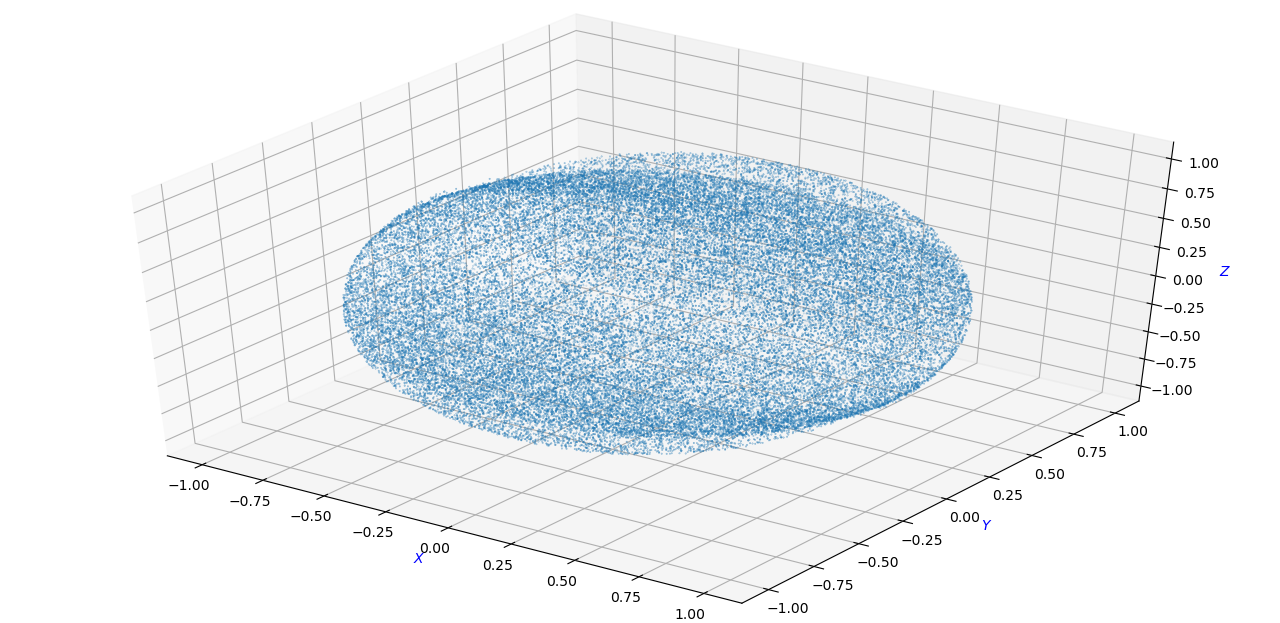
\includegraphics[width=0.45\textwidth]{../4-xyz.png}}
			\subfigure[$N=10000$二维投影]{
				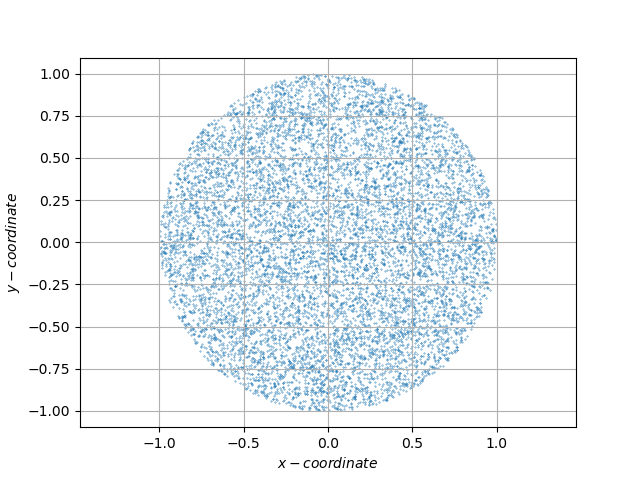
\includegraphics[width=0.45\textwidth]{../4-xy-1w.png}}
			\subfigure[$N=50000$二维投影]{
				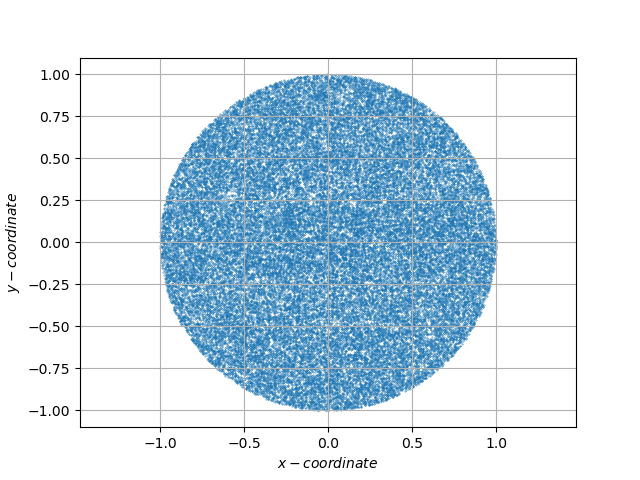
\includegraphics[width=0.45\textwidth]{../4-xy.png}}
			\caption{四维投影分布}
		\end{figure}
\begin{flushleft}
		可见,三维投影更像是两个球体交叠在一起,在二维上投影均匀性比之前三维球面分布要高很多。
\end{flushleft}

尽管使用$Masarglia$抽样可以不断得到更高维的球面上均匀分布,但是效率在逐步下降,直观上因为高维球体占据外接正方体体积比逐步下降,使得舍选效率降低。

\begin{table}[H]
	\centering
	\setlength{\tabcolsep}{20mm}{
		\begin{tabular}{@{}cl@{}}
			\toprule
			$dimension$&$ratio$ \\ \midrule
			$1d$&1.000000 \\
			$ 2d $&0.785398\\
			$ 3d $&0.523599	\\
		$ 	4d $&0.308425	 \\ \bottomrule
			
	\end{tabular}}
	\caption{高维球体体积占据比}
\end{table}
	\clearpage
	\section{总结}
	\begin{itemize}
		\item $Marsaglia$抽样法在难以通过直接抽样和变换抽样法时不失为一种有效的抽样方法。但是它的缺点也是所以舍选抽样具有的,效率问题。对于特别高维的球面均匀分布如果还使用$Marsaglia$抽样很多时候会抽到舍弃点,效率低。
	\end{itemize}
	\clearpage
\end{document}